\subsection{Определение эффективности отбора}



\subsubsection{Моделирование}

\begin{figure}
	\centering
	\label{fig:cm12mc}
	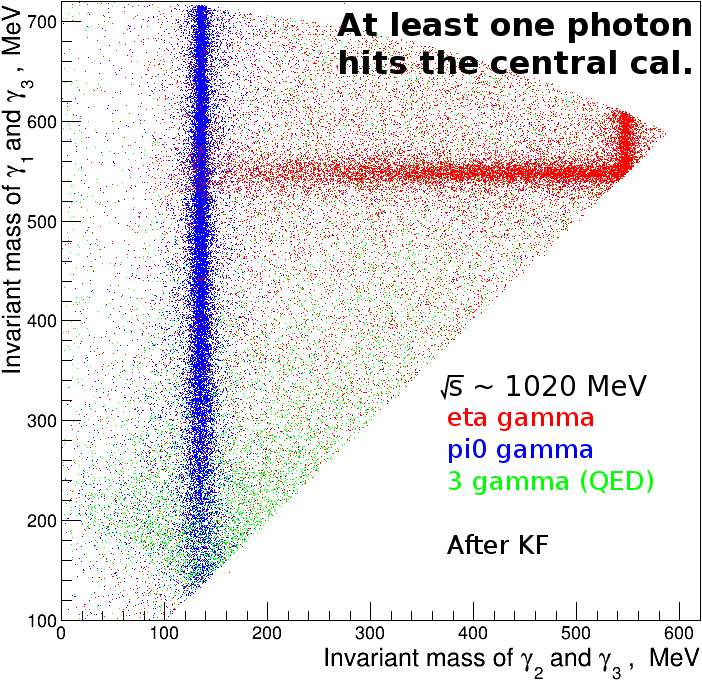
\includegraphics[width=.5\textwidth]{img/cm12mc.png}
	\caption{Диаграмма Далица после КР 
			для событий моделирования в области $\phi$-мезона
			$e^+ e^- \to \pi^0 \gamma$ (синие точки),
			$e^+ e^- \to \eta \gamma$ (красные точки)
			и трёхквантовой аннигиляции (зелёные точки),
			когда хотя бы один фотон попал в \ce{LXe} калориметр.}
\end{figure}

Для определения эффективности отбора событий $e^+ e^- \to \pi^0 \gamma, \, \eta \gamma$ по конченому трёхфотонному состоянию разработанный метод применялся к данным моделирования.
Моделирование проводилось с помощью пакета \emph{GEANT4}, \cite{geant4Allison:2006ve}.
Пример диаграммы Далица приведён на рисунке~\ref{fig:cm12mc}.
В моделирование учитывались все возможные каналы распадов псевдоскалярных мезонов, также моделирование идёт с излучением радиационных фотонов.
На рисунках \textbf{пара рисунков с эффективностью от с.м. энергии} представлены эффективности при разных условиях отбора в зависимости от полной энергии в системе центра масс.

Падение эффективности с ростом энергии объясняется увеличением вероятности иметь маленькие углы между фотонами в событие,
что приводит к сливанию электромагнитных ливней в калориметре детектора.

Вблизи порога реакции $e^+ e^- \to \eta \gamma$ монохроматичный фотон становится мягким, что уменьшает вероятность регистрации.
Так начиная при энергии системы $\sqrt{s} = \SI{666}{\MeVr}$ энергия монохроматичного фотона равна \SI{30}{\MeVr}, что соответствует порогу на рассмотрения фотона как значащего.

% Для определения эффективности разработанного метода применялся на данных моделирования $e^+ e^- \to
% \eta \gamma$ и $e^+ e^- \to \pi^0 \gamma$.
% Причём с распадом псевдоскалярных мезон во все возможные каналы.
Так характерная эффективность в области $\phi$-мезона без ограничения на углы вылета конечных
фотонов составила \SI{23.7}{\percent} для $\eta \gamma$ процесса.
Для $\pi^0 \gamma$ при условии попадания хотя бы одного фотона в центральную часть детектора
составляет приблизительно \SI{5}{\percent},
при этом наблюдается спад эффективности с ростом $\sqrt{s}$.



\subsubsection{Поправка к эффективности регистрации фотонов}



Эффективность реконструкции фотонов в моделировании и эксперименте определено по событиям процесса
$e^+ e^- \to \pi^+ \pi^- \pi^0 \to \pi^+ \pi^- 2 \gamma$.
Отобранные события разбиваются на два класса:
событие полностью реконструировано и
события с одним потерянным фотоном.


\paragraph{Отбор событий $e^+ e^- \to \pi^+ \pi^- \pi^0$}

На первом этапе отбираются события с двумя центральными треками и с одним или двумя фотонами.
Так же требуется, чтобы флаг is\_bhabha не равнялся 1.
От трека требуется наличие кластера с полярным углом удовлетворяющем условию $0.9 < \theta < \pi - 0.9$.

Для треков определяется отношение энерговыделения к импульсу и
требуется,
чтобы каждое $E_{dep} / p$ лежало в диапазоне $(0.1, \, 2)$.

На каждый фотон накладываются условия:
\begin{itemize}
    \item $| \theta - \pi/2| < 1.4 \approx \ang{80.214}$,
    \item $\SI{15}{\MeVr} < E < 0.75 \sqrt{s}$.
\end{itemize}
После этого должно остаться один или два фотона, чтобы событие осталось в обработке.

Для отобранных частиц вычисляется модуль полного импульса системы $P_{tot}$ и полная энергия $E_{tot}$:
\begin{align}
    E_{tot} &= \sum E_i , \\
    P_{tot} &= \left| \vec{P}_{tot} \right| = \left| \sum \vec{p}_i \right| .
\end{align}
На ни накладываются следующие условия:
\begin{itemize}
    \item $P_{tot} < 0.75 \sqrt{s}$,
    \item $0.25 \sqrt{s} < E_{tot} < 1.75 \sqrt{s}$.
\end{itemize}
\begin{figure}[htbp]
    \centering
    \begin{subfigure}[b]{0.45\textwidth}
        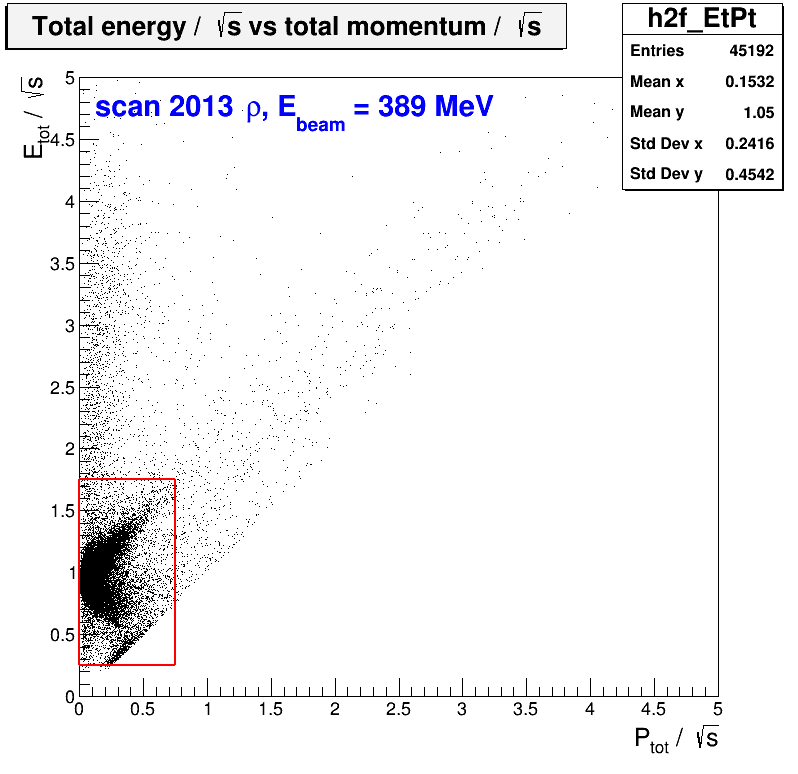
\includegraphics[width=\textwidth]{img/h2f_EtPt.png}
        \caption{Полный вид.}
        \label{fig:EtPt_full}
    \end{subfigure}
    ~
    \begin{subfigure}[b]{0.45\textwidth}
        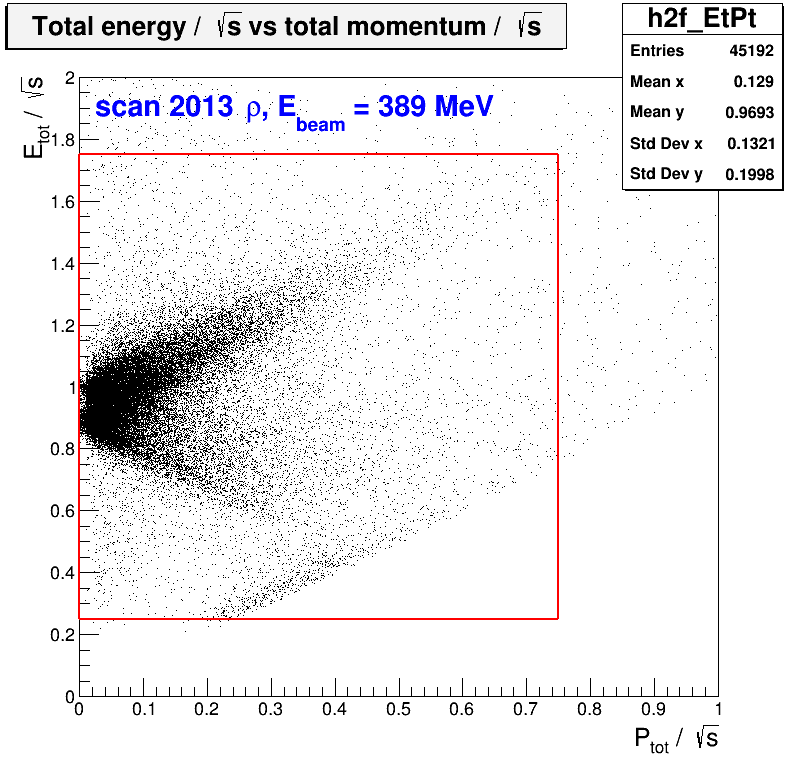
\includegraphics[width=\textwidth]{img/h2f_EtPt_zoom.png}
        \caption{Область выбора приближена.}
        \label{fig:EtPt_zoom}
    \end{subfigure}
    \caption{Распределение полной энергии и полного импульса системы,
        нормированные на $\sqrt{s}$.
        Красной линией обозначены условия отбора.
        Экспериментальные данные сезона $2013 \, \rho$,
        $E_{beam} = \SI{389}{\MeVr}$.}\label{fig:EtPt}
\end{figure}

Для прошедших отборы событий проводится кинематическая реконструкция в гипотезе четырёх частиц (двух заряженных пионов и двух фотонов) с требованием выполнения законов сохранения импульса-энергии для всей системы.
Таким образом после кинематической реконструкции суммарный импульс системы $P^{KF}_{tot}$ стремится к нулю,
а общая энергия системы $E^{KF}_{tot}$ к энергии двух пучков.
\begin{figure}[htbp]
    \centering
    \begin{subfigure}[t]{0.45\textwidth}
        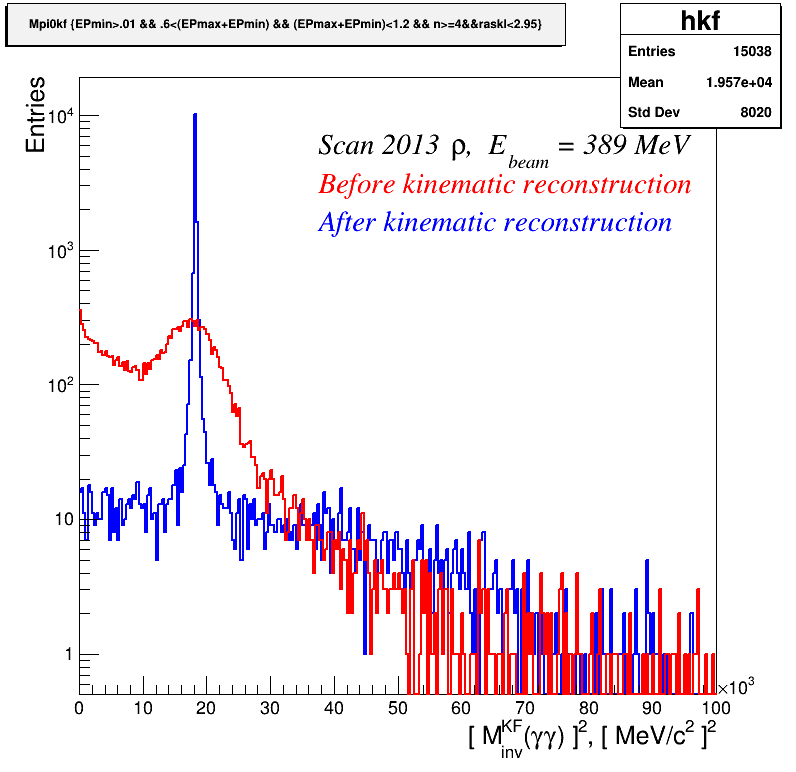
\includegraphics[width=\textwidth]{img/diff_kf_mpi0_2013rho389.png}
        \caption{Данные сезона $2013 \, \rho$, $E_{beam} = \SI{389}{\MeVr}$.}
        \label{fig:diff_kf_mpi0_2013rho389}
    \end{subfigure}
    ~
    \begin{subfigure}[t]{0.45\textwidth}
        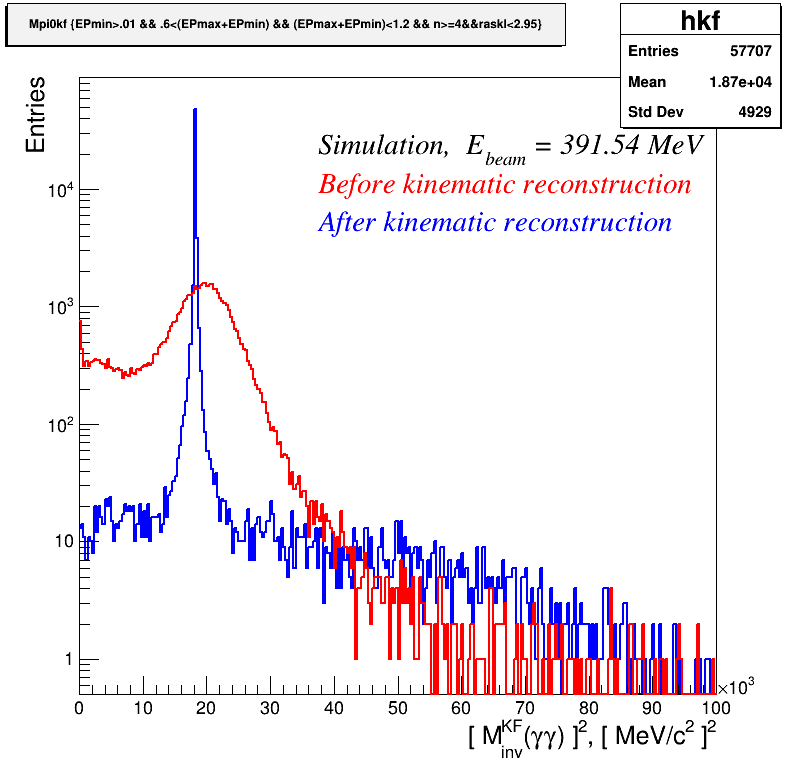
\includegraphics[width=\textwidth]{img/diff_kf_mpi0_sim391_54.png}
        \caption{Моделирование $e^+ e^- \to \pi^+ \pi^- \pi^0$, $E_{beam} = \SI{391.54}{\MeVr}$.}
        \label{fig:diff_kf_mpi0_sim391_54}
    \end{subfigure}
    \caption{Распределение событий по квадрату инвариантной массы двух фотонов для событий с двумя и более фотонами.
    Красная (синяя) гистограмма --- до (после) кинематической реконструкции.}\label{fig:diff_kf_mpi0}
\end{figure}

 
Второй этап отборов начинается с требования на массу отдачи двух заряженных пионов $M_{recoil}^{\pi^+ \pi^-}$,
а именно $\SI{0}{\MeVr} < M_{recoil}^{\pi^+ \pi^-} < \SI{300}{\MeVr}$.
Дополнительно для треков накладывается условие
% $ 0.1 < E_1/p_1 , \, E_2/p_2 < 2 $.
$ E_1/p_1 + E_2 / p_2 < 1$
и $\min(E_i / p_i) > 0.1$.
В то время как на угол между треками $\Omega_{\pi^+ \pi^-}$ накладывается условие $\Omega_{\pi^+ \pi^-} < 2.95$.
Данное условие продемонстрировано на рисунках~\ref{fig:raskl}.
\begin{figure}
    \begin{minipage}[t]{0.45\textwidth}
        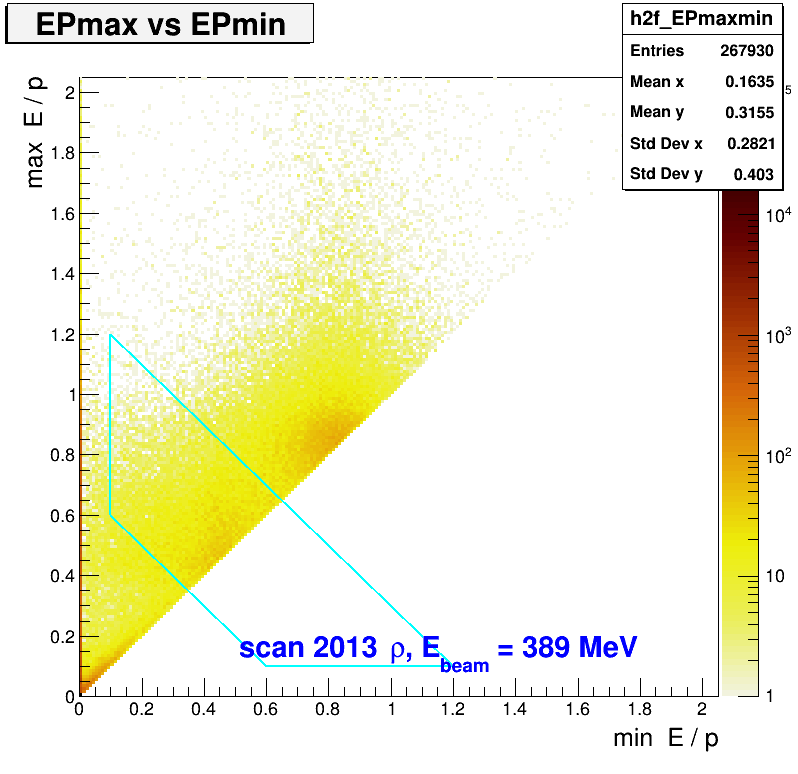
\includegraphics[width=\textwidth]{img/h2f_EPmaxmin_zoom.png}
        \caption{Распределение отношения энерговыделения трека к импульсу трека.
            Голубой линией обозначены условия отбора по $E_i / p_i$.
            Экспериментальные данные сезона $2013 \, \rho$, $E_{beam} = \SI{394}{\MeVr}$.}
        \label{fig:EPmaxmin_zoom}
    \end{minipage}
    \qquad
    \begin{minipage}[t]{0.45\textwidth}
        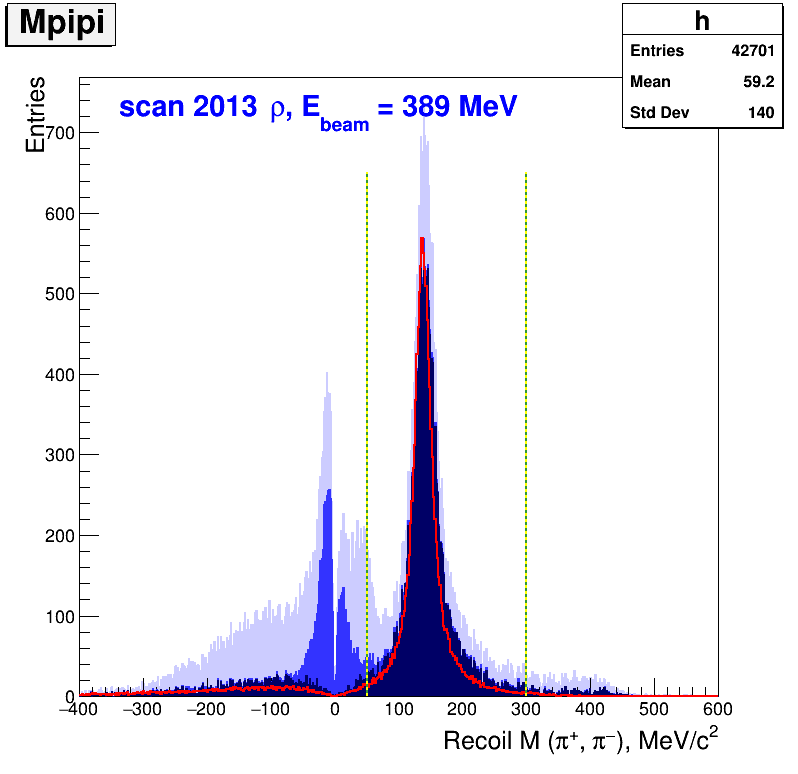
\includegraphics[width=\textwidth]{img/mpipi.png}
        \caption{Тёмно-синяя гистограмма --- с отбором по $E/p$ и $\Omega_{\pi^+ \pi^-}$,
            синяя гистограмма --- с отбором по $E/p$,
            блеклая гистограмма --- до отбора по $E/p$,
            красная линия --- моделирование после отбора по $E/p$ и $\Omega_{\pi^+ \pi^-}$,
            зелёно-жёлтая штрихованная линии --- условия отбора по $M_{recoil}^{\pi^+ \pi^-}$.}
        \label{fig:mpipi}
  \end{minipage}
\end{figure}


\begin{figure}[htbp]
    \centering
    \begin{subfigure}[b]{0.45\textwidth}
        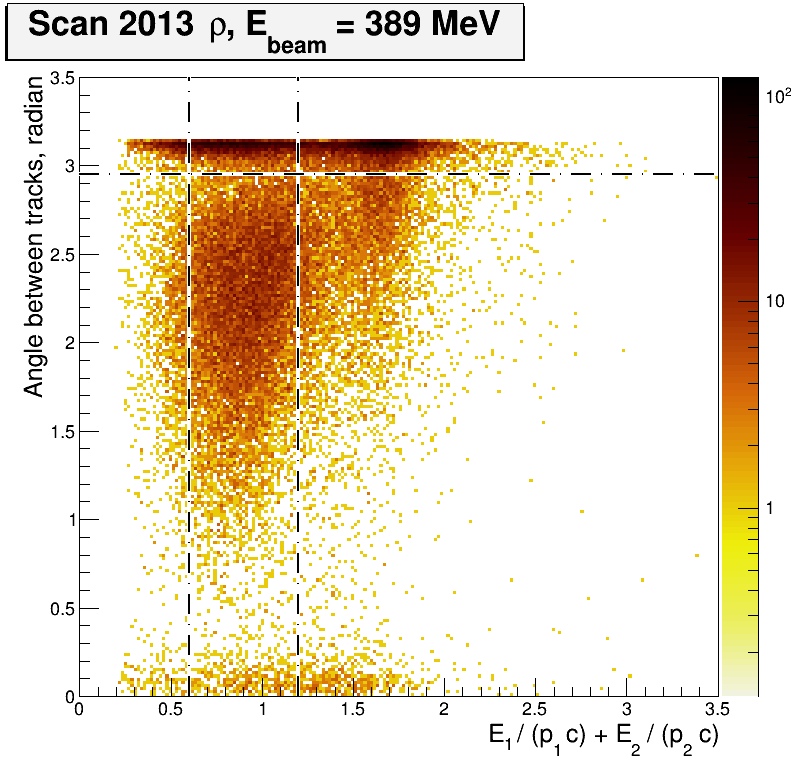
\includegraphics[width=\textwidth]{img/raskl_vs_sumEP_rho389.png}
        \caption{Данные сезона $2013 \, \rho$, $E_{beam} = \SI{389}{\MeVr}$.}
        \label{fig:raskl_rho389}
    \end{subfigure}
    ~
    \begin{subfigure}[b]{0.45\textwidth}
        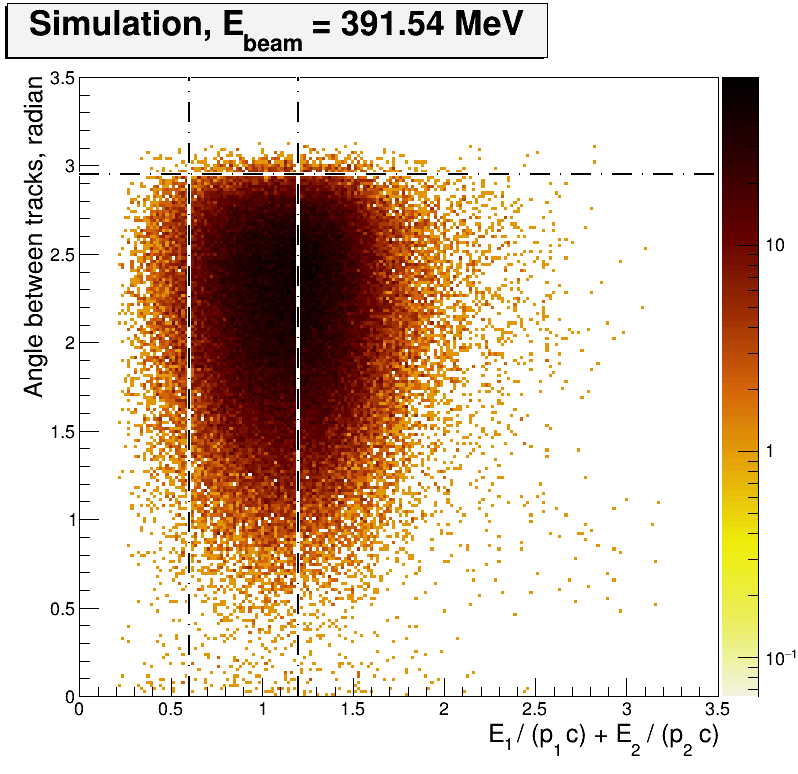
\includegraphics[width=\textwidth]{img/raskl_vs_sumEP_sim391_54.png}
        \caption{Simulation $\pi^+ \pi^- \pi^0$, $E_{beam} = \SI{391.54}{\MeVr}$.}
        \label{fig:raskl_sim391_54}
    \end{subfigure}
    \caption{Distribution of an angle between tracks $\Omega_{\pi^+ \pi^-}$ versus $E_1/p_1 + E_2 / p_2 < 1$.
    Vertical lines represent the used cut on $\sum E_i / p_i$.}\label{fig:raskl}
\end{figure}




\subsubsection{Эффективность триггера}

Вычисление сечений изучаемых реакций требует учёта эффективности нейтрального триггера $\varepsilon_{NT}$,
которая извлекается по событиям радиационного баба рассеяния $e^+e^- \to e^+e^-\gamma$.


Процесс $e^+e^- \to e^+e^-\gamma$ выбран по ряду причин.
Он похож по характеру энерговыделения,
так как и фотоны,
и электроны рождают электромагнитный ливни.
Количество частиц в конечном состоянии равно оному в изучаемых процессах,
а именно трём.
Из первых двух пунктов следует,
что и система нейтрального триггера будет реагировать похожим образом
---
срабатывают те же маски.
В процессе есть как заряженные,
так и нейтральная частицы,
что позволяет использовать две независимые подсистемы запуска детектора,
позволяющие изучать вероятность срабатывания друг друга.
% что позволяет использовать особенности триггера детектора КМД-3
% ---
% две независимых подсистемы запуска детектора.
Сечение процесса $e^+e^- \to e^+e^-\gamma$ плавное и достаточно велико во всей доступной области энергий.


Отбираются события с двумя центральными треками и хотя бы одним фотоном,
при этом на гамма-кванты налагаются дополнительные условия, 
как $0.42 < \theta < \pi - 0.42$, 
так и $E_\gamma > \SI{30}{\MeVr}$.
Центральным треком
---
треком лежащим в том числе в области взаимодействия пучков или рядом с ней
---
считается такой трек,
который удовлетворяет следующим условиям:
\begin{itemize}
	\item максимально расстояние между треком и орбитой пучков не более \SI{6}{\cmr} в плоскоти $\rho-\varphi$;
	\item $\chi^2_{R} < 100$ из подгонки хитов ДК в $\rho$--$\varphi$ плоскости;
	\item $\chi^2_{Z} < 100$ из подгонки хитов ДК в $\rho$--$z$ плоскости.
\end{itemize}
Более того требуется, чтобы хотя бы одна из частиц летела в цилиндрический калориметр:
$ 0.9 < \theta < \pi - 0.9 $.
Последние условие,
как правило,
обеспечивается одним из треков,
ввиду неэффективности восстановления треков при малых полярных углах.

Затем для каждого события вычисляется полная энергия $E_{sys}$ и полный импульс $P_{sys}$ системы частиц,
причём для нейтральных частиц импульс приравнивается к их энергии, а энергия заряженных частиц рассчитывается как $E = \sqrt{p^2 + {m_e}^2}$.
Таким образом последние частицы предполагаются электронами или позитронами с массой $m_e$.
На полный импульс $P_{sys}$ и полную энергию $E_{sys}$ полученной системы частиц накладываются нижеприведённые условия:
\begin{itemize}
    \item $P_{sys} < 0.25 \sqrt{s}$;
    \item $\frac{2}{3} \sqrt{s} + P_{sys} < E_{sys} < 1.25 \sqrt{s}$.
\end{itemize}
Для определения эффективности триггера отбираются события с $\min (E/p) > 0.8$ и $\max (E/p) < 2$.
Такое условие позволяет дополнительно подавить
фон от минимально ионизирующих частиц $\pi^\pm$ и $\mu^\pm$.
при этом происходят два вида отборов с количеством летящих в цилиндрическую часть детектора частиц:
не меньшим одного и не меньше трёх.


Дополнительно для каждого события сохраняется информация о том,
какой из триггеров сработал:
\begin{itemize}
  \item нейтральный триггер;
  \item заряженный триггер;
  \item полный триггер, то есть в событие сработал и заряженный, и нейтральный триггер.
\end{itemize}
Теперь для каждой точки по энергии определяются количества событий, в которых сработал:
\begin{itemize}
  \item только нейтральный триггер --- $N_{NT}$;
  \item только заряженный триггер ---  $N_{CT}$;
  \item полный триггер --- $N_{tot}$.
\end{itemize}
На основе этих данных рассчитывается эффективности нейтрального триггера $\varepsilon_{NT}$,
заряженного триггера $\varepsilon_{CT}$ и полного триггера $\varepsilon_{tot}$.
Пусть произошло $N$ событий $e^+ e^- \to e^+ e^- \gamma$,
тогда можно записать систему уравнений:
\begin{align}
    N_{NT} &= \varepsilon_{NT} \cdot ( 1 - \varepsilon_{CT} ) \cdot N , \\
    N_{CT} &= ( 1 - \varepsilon_{NT} ) \cdot \varepsilon_{CT} \cdot N , \\
    N_{NT} &= \varepsilon_{NT} \cdot \varepsilon_{CT} \cdot N .
\end{align}
Разрешим данные связи относительно искомых эффективностей:
\begin{align}
    \varepsilon_{NT} &= \frac{ N_{tot} }{ N_{tot}+N_{CT} } , \\
    \varepsilon_{CT} &= \frac{ N_{tot} }{ N_{tot}+N_{NT} } , \\
    \varepsilon_{tot} &= 
    \frac{ N_{tot} (N_{tot}+N_{CT}+N_{NT}) }{
        (N_{tot}+N_{CT}) (N_{tot}+N_{NT})
    } \\
    &=
    1 - (1-\varepsilon_{NT}) (1-\varepsilon_{CT}) .
\end{align}
Положив статистическую неопределённость $N_i$,
где $i = NT, \, CT,$ и $tot$,
равными $ \Delta N_i  = \sqrt{N_i} $ можно вычислить погрешности определения эффективностей,
воспользовавшись формулой переноса ошибок.
\[ \Delta  \varepsilon_{NT} = \frac{1}{ ( N_{TC} + N_T )^2} \left[ N_{TC}  N_T ( N_{TC} + N_T )
\right]^\frac{1}{2} \]
\[ \Delta  \varepsilon_{CT} = \frac{1}{ ( N_{TC} + N_C )^2} \left[ N_{TC}  N_C ( N_{TC} + N_C )
\right]^\frac{1}{2} \]
\[ \Delta  \varepsilon_{tot} =  \left[ (1-\varepsilon_{NT})^2 {\Delta  \varepsilon_{CT}}^2 +
(1-\varepsilon_{CT})^2 {\Delta  \varepsilon_{NT}}^2 \right]^\frac{1}{2} \]

Основными фоновыми процессам для $e^+ e^- \to e^+ e^-\gamma$ являются процессы $e^+ e^- \to \pi^+ \pi^- \gamma$ и $e^+ e^- \to \pi^+ \pi^- \pi^0 \to \pi^+ \pi^- 2\gamma$.
Так как эти процессы носят резонансный характер, то их вклад в ошибку определения эффективности триггера будет наиболее большим в области $\omega (782)$ и $\phi (1020)$ резонансов.
Для подавление событий с заряженными пионами используется ограничение на отношение импульса частицы, измеренного трековой системой детектора, к энергии, определённой по данным калориметра.
Для электронов и позитронов это отношение близко к единице.
В случае пионов оно пикуются в области $P/E = \sqrt{1 - {m_{\pi^\pm}}^2 / E^2}$, так для энергии пиона равной $300$~МэВ расчётное $P/E \simeq 0.88$.

Далее определялась эффективность нейтрального триггера, а также заряженного и полного, в зависимости от диапазона полярных углов частиц.
Будем накладывать ограничение на минимальный угол $\theta_{min}$ между частицами и осью пучков.
Из рисунка \textbf{рисунок} видно, что начиная с $\theta_{min} = 0.9$ эффективность стабилизируется и перестаёт зависеть от $\theta_{min}$, далее для определения эффективности триггера будет использоваться именно это значение минимального угла.

Теперь определим эффективности триггеров для всей статистики, используемой в данной работе.
На рисунке~\ref{fig:nt_eff} представленность зависимость эффективностей от энергии в системе центра масс.
Видно, что области резонансов наблюдаются некоторые провалы в эффективностях, наиболее ярко это видно для заряженного триггера.


\begin{figure}
    \centering
    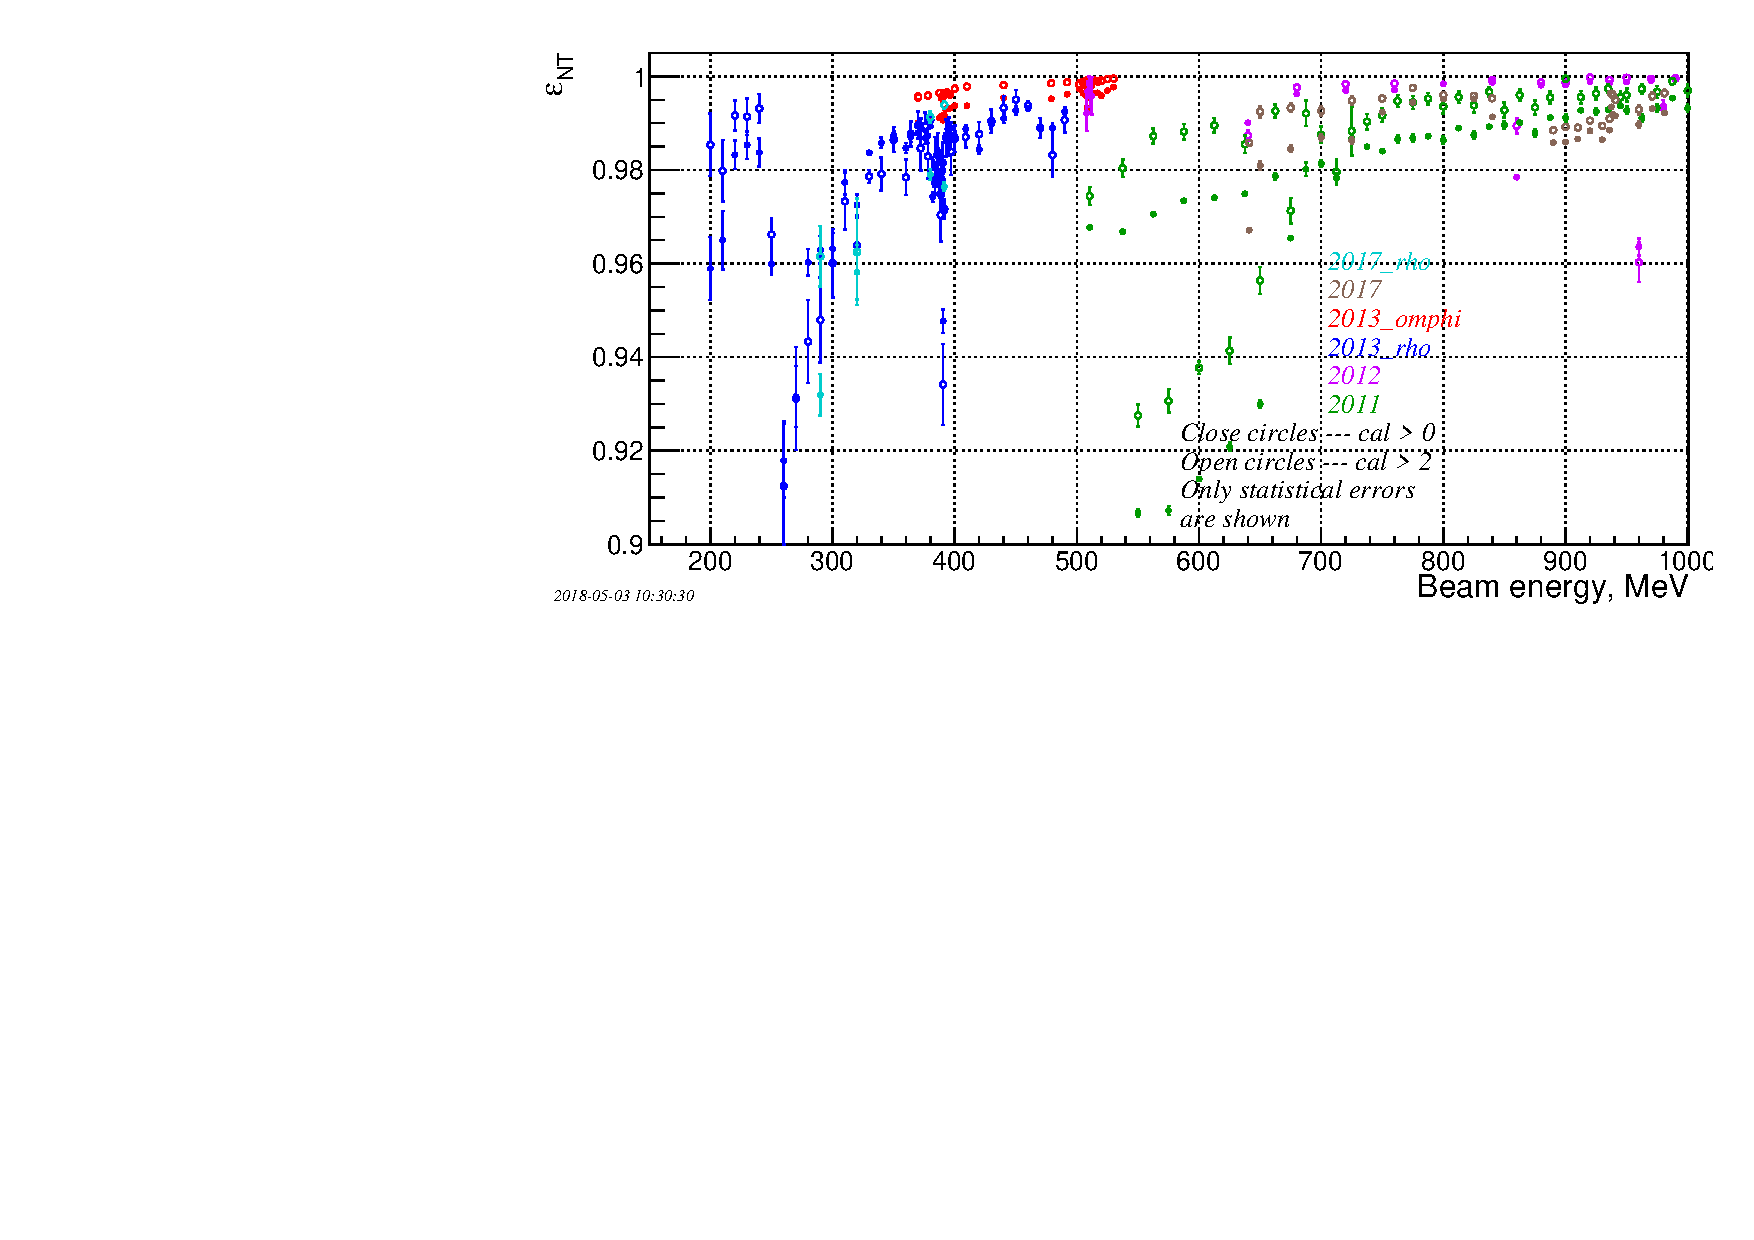
\includegraphics[width=\textwidth]{img/nt_eff.pdf}
    \caption{Эффективность нейтрального триггера.}
    \label{fig:nt_eff}
\end{figure}



\subsubsection{Учёт радиационных поправок}